\documentclass[12pt]{article}
\usepackage[a4paper, total={6in, 10in}]{geometry}
\usepackage[utf8]{inputenc}
\usepackage{caption}
\usepackage{amsmath}
\usepackage{amssymb}
\usepackage{mathtools}
\usepackage{multicol}
\usepackage{mhchem}
\usepackage{graphicx}
\usepackage{wrapfig}
\usepackage{float}
\usepackage{makecell}
\usepackage[makeroom]{cancel}

\graphicspath{ {./images/} }

\renewcommand{\baselinestretch}{1.5} % line spacing
\newcommand{\fline}{\par\noindent\rule{\textwidth}{0.1pt}} % horizontal line (wide)

\title{2D Collision Momentum Lab}
\author{Peter Zhang}

\begin{document}

\maketitle
\newpage


\section{Purpose}
To investigate the conservation of momentum in a 2D collision and determine if the collision is elastic.

\section{Data Tables}

\begin{center}
\begin{tabular}{|c|c|}
\hline
Variable & Measured Value\\
\hline
\hline
$m_{ball\ 1+2}$ & $28.4 \pm 0.2g$\\
\hline
$h_{table}$ & $75.5\pm0.1cm$\\
\hline
$h_{ramp}$ & $15.2\pm0.1cm$\\
\hline
$\triangle{d}_{X\rightarrow{}T_{1}}$ & $11.4\pm0.1cm$\\
\hline
$\triangle{d}_{X\rightarrow{}I_{1}}$ & $40.4\pm0.1cm$\\
\hline
\end{tabular}
\captionof{table}{Measured Values}

\begin{tabular}{|c|c|}
\hline
Variable & Value\\
\hline
\hline
$\theta{}_{T_{1}} $ & $0.90\pm0.04rad$\\
\hline
$\theta{}_{I_{1}} $ & $0.292\pm0.006rad$\\
\hline
$\triangle{t_{table\rightarrow ground}}$ & $0.3925\pm0.0003s$\\
\hline
$\vec{v_{ball\ 1}^{'}} \ce{(part 1)}$ & $1.726\pm0.006m/s\ [(+)\ x-axis]$\\
\hline
$\vec{v_{ball\ 1}^{'}} \ce{(part 2)}$ & $0.367\pm0.003m/s\ [0.90\pm0.04rad\ \ce{above x-axis in z-plane}]$\\
\hline
$v_{ball\ 1,\ x}^{'} \ce{(part 2)}$ & $0.23\pm0.01m/s$\\
\hline
$\vec{v_{ball\ 2}^{'}} \ce{(part 2)}$ & $1.029\pm0.003m/s\ [0.292\pm0.06rad\ \ce{below x-axis in z-plane}]$\\
\hline
$v_{ball\ 2,\ x}^{'} \ce{(part 2)}$ & $0.99\pm0.06m/s$\\
\hline
\end{tabular}
\captionof{table}{Calculated Values}

\end{center}

\pagebreak

\section{Experiment Diagram}

\begin{figure}[H]
\centering
\fbox{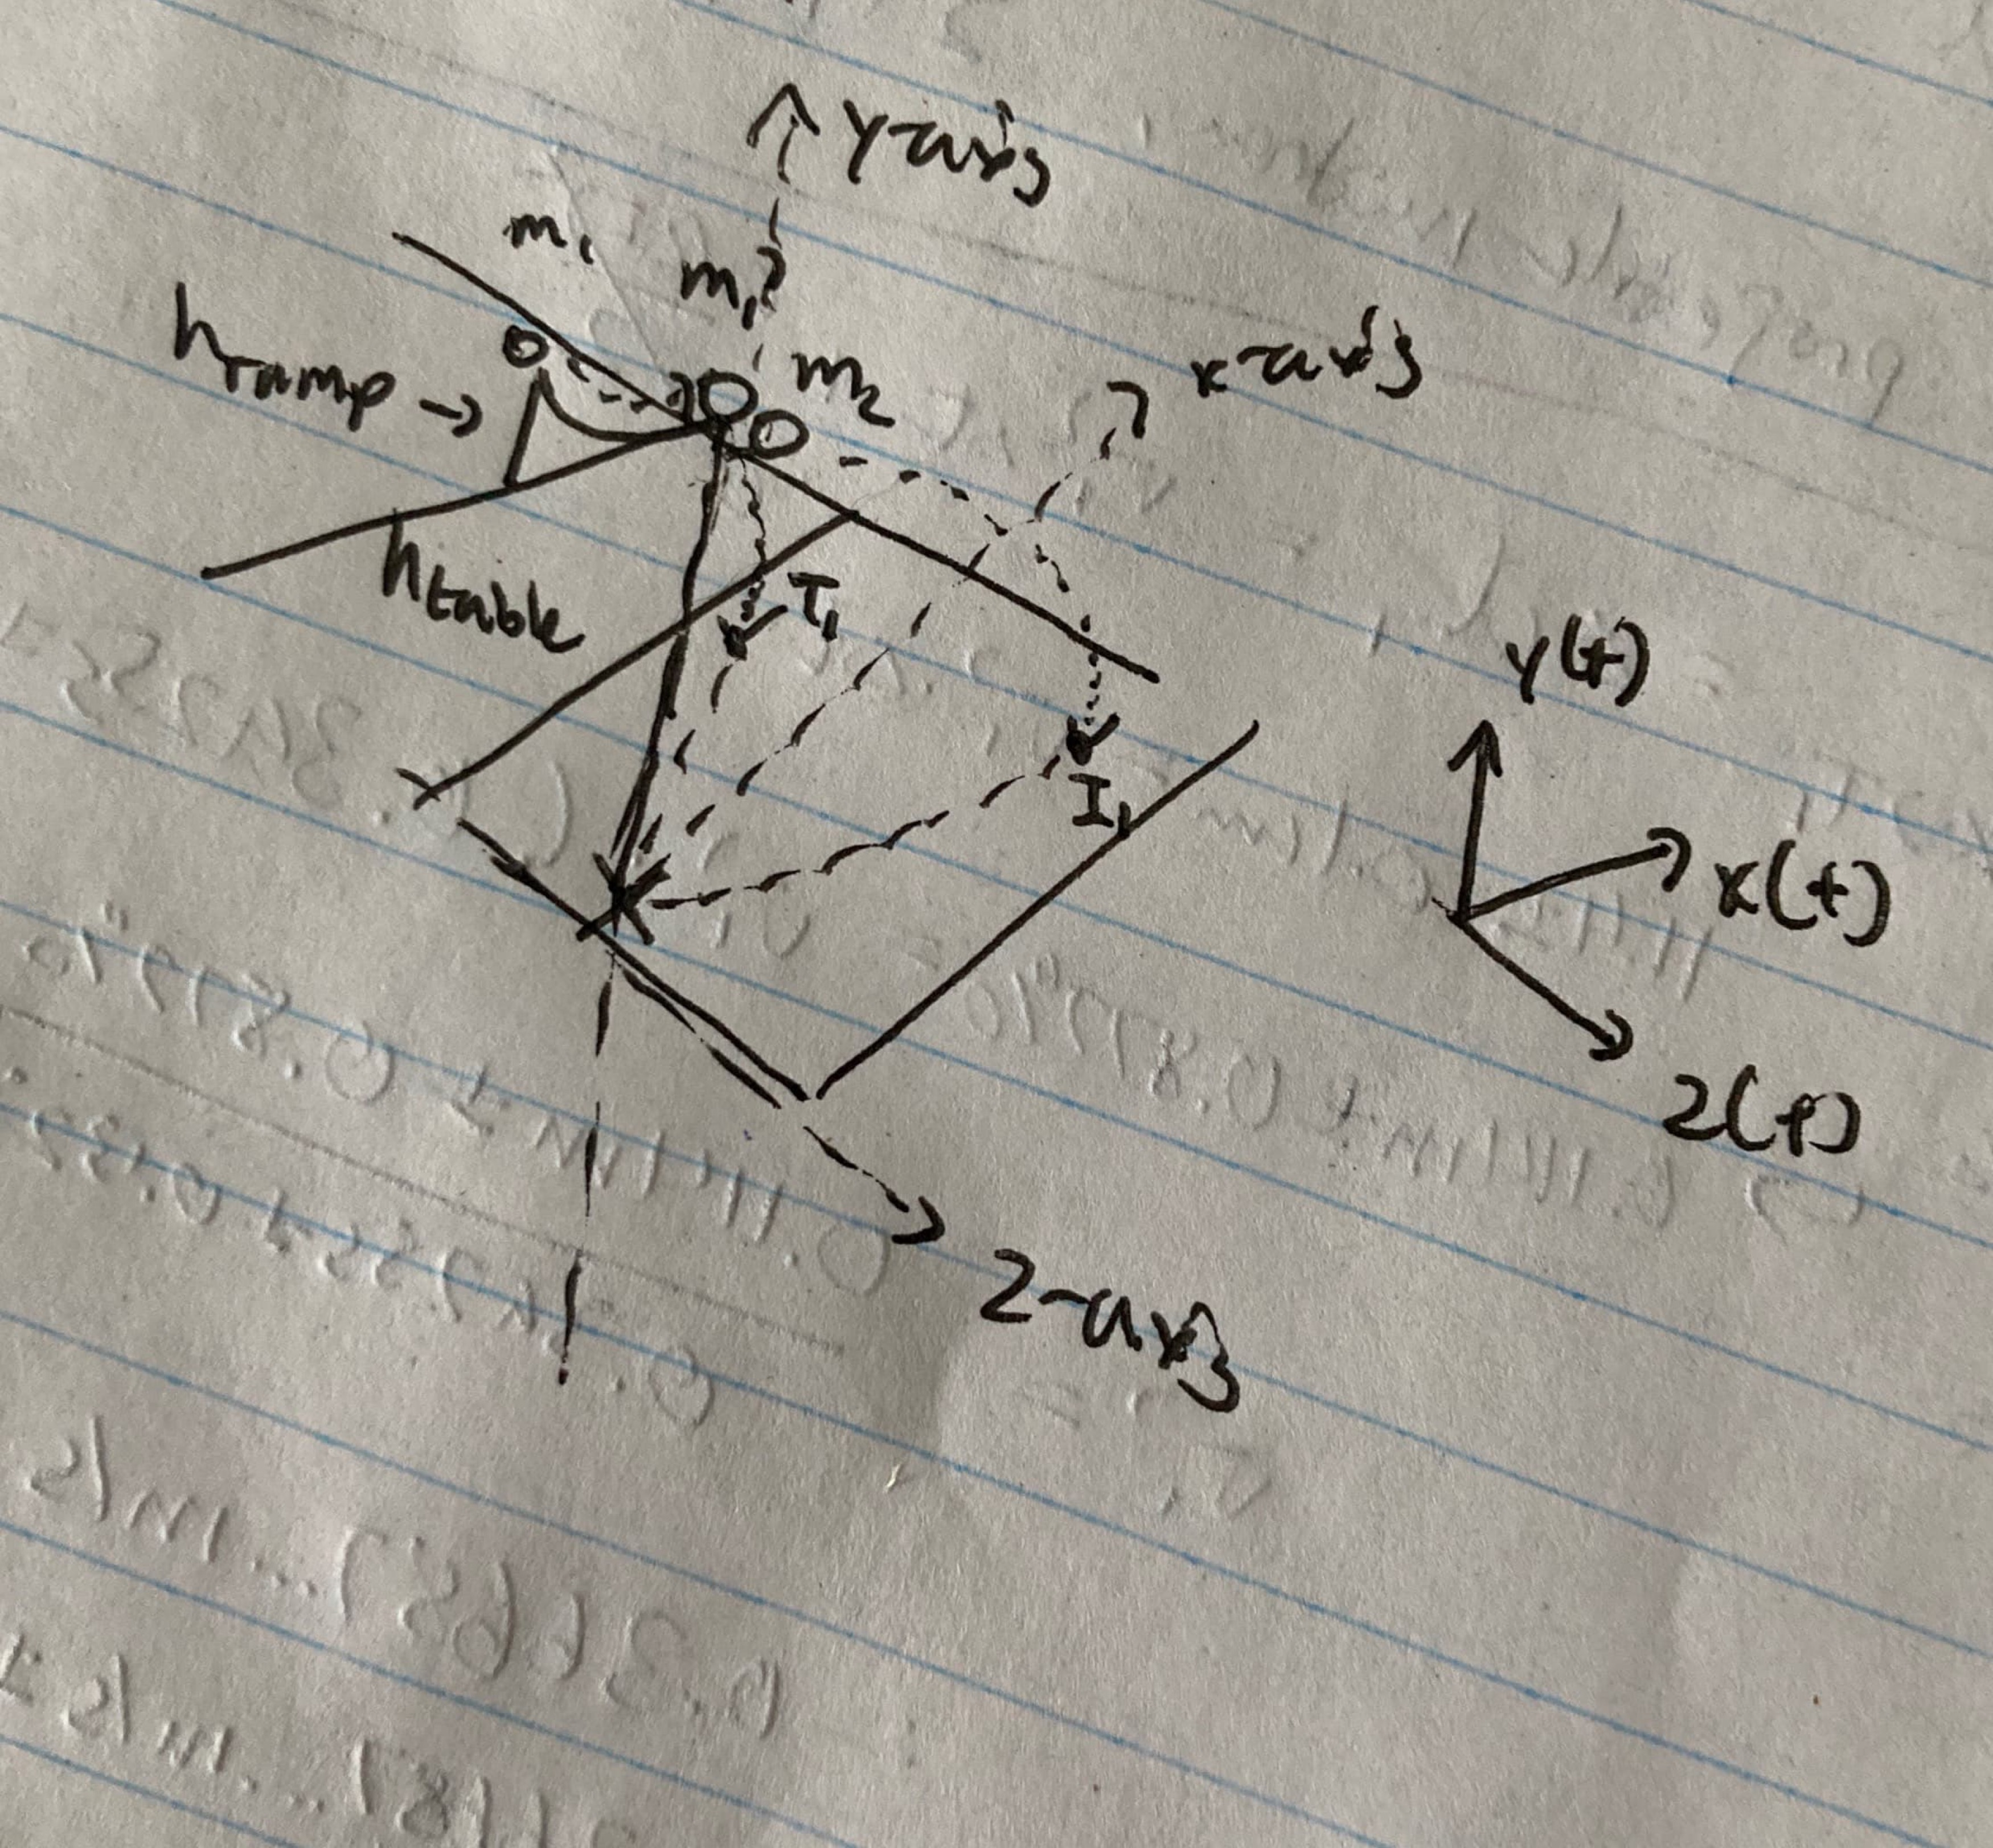
\includegraphics[width=\textwidth]{ExperimentDiagram.jpg}}
\captionof{figure}{Diagram of the Experiment}
\end{figure}

\pagebreak

\section{Analysis}
\subsection{Question 1}
Draw a line and measure the distance from point X to point T1 and from point X to point I1. 

\begin{center}
\begin{figure}[H]
\centering
\fbox{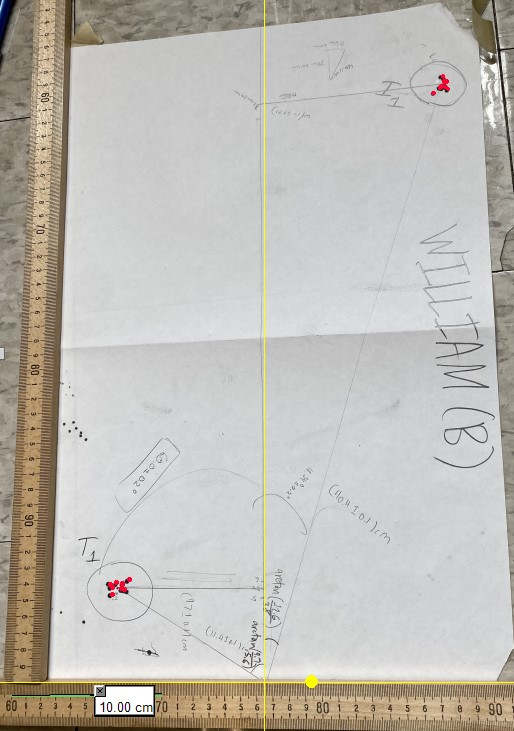
\includegraphics[width=300pt]{landingpoints.jpg}}
\captionof{figure}{Landing Points}
\end{figure}
\end{center}

Using a ruler, we measured the distances to be $\triangle{d}_{X\rightarrow{}T_{1}} = 11.4\pm0.1cm$ and $\triangle{d}_{X\rightarrow{}I_{1}} = 40.4\pm0.1cm$. 

\pagebreak

\subsection{Question 2}
Determine the angle between the line XT1 and the x-axis as well as between XI1 and x-axis. Mention the method by which you determine the angles and show work if necassary.

\subsubsection{Calculating for $T_{1}$ and $I_{1}$}
Inserting the following data into Logger Pro:
\begin{center}
\begin{figure}[H]
\centering
\fbox{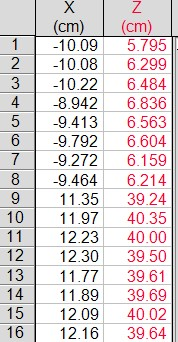
\includegraphics[width=150pt]{datapoints.jpg}}
\captionof{figure}{Image Analysis Landing Points Relative to \textbf{Point X}\\First 8 (for $T_{1}$) Next 8 (for $I_{1}$)}
\end{figure}
\end{center}
Using this data and a GDC, can be made to find the average of these points. $T_{1} = (6.369\pm0.301cm, -9.659\pm0.427cm)$ and $I_{1} = (39.756\pm0.327cm, 11.958\pm0.280cm)$. We can then calculate for $\theta{}$ using the trigonometric relationship $\tan{\theta{}} = \ce{\frac{opp}{adj}}$.

\pagebreak
\subsubsection{Solving for Angles}
The percent uncertainty for:\\
$\sigma{}T_{1x} = \frac{0.301cm}{6.369cm} \cdot{} 100\% = \pm4.73\%$\\
$\sigma{}T_{1y} = \frac{0.427cm}{-9.659cm} \cdot{} 100\% = \pm4.42\%$\\
$\sigma{}I_{1x} = \frac{0.327cm}{39.756cm} \cdot{} 100\% = \pm0.823\%$\\
$\sigma{}I_{1y} = \frac{0.280cm}{11.958cm} \cdot{} 100\% = \pm2.34\%$


\begin{center}

\begin{tabular}{c l}
\hline
\raisebox{-0.5\totalheight}{\fbox{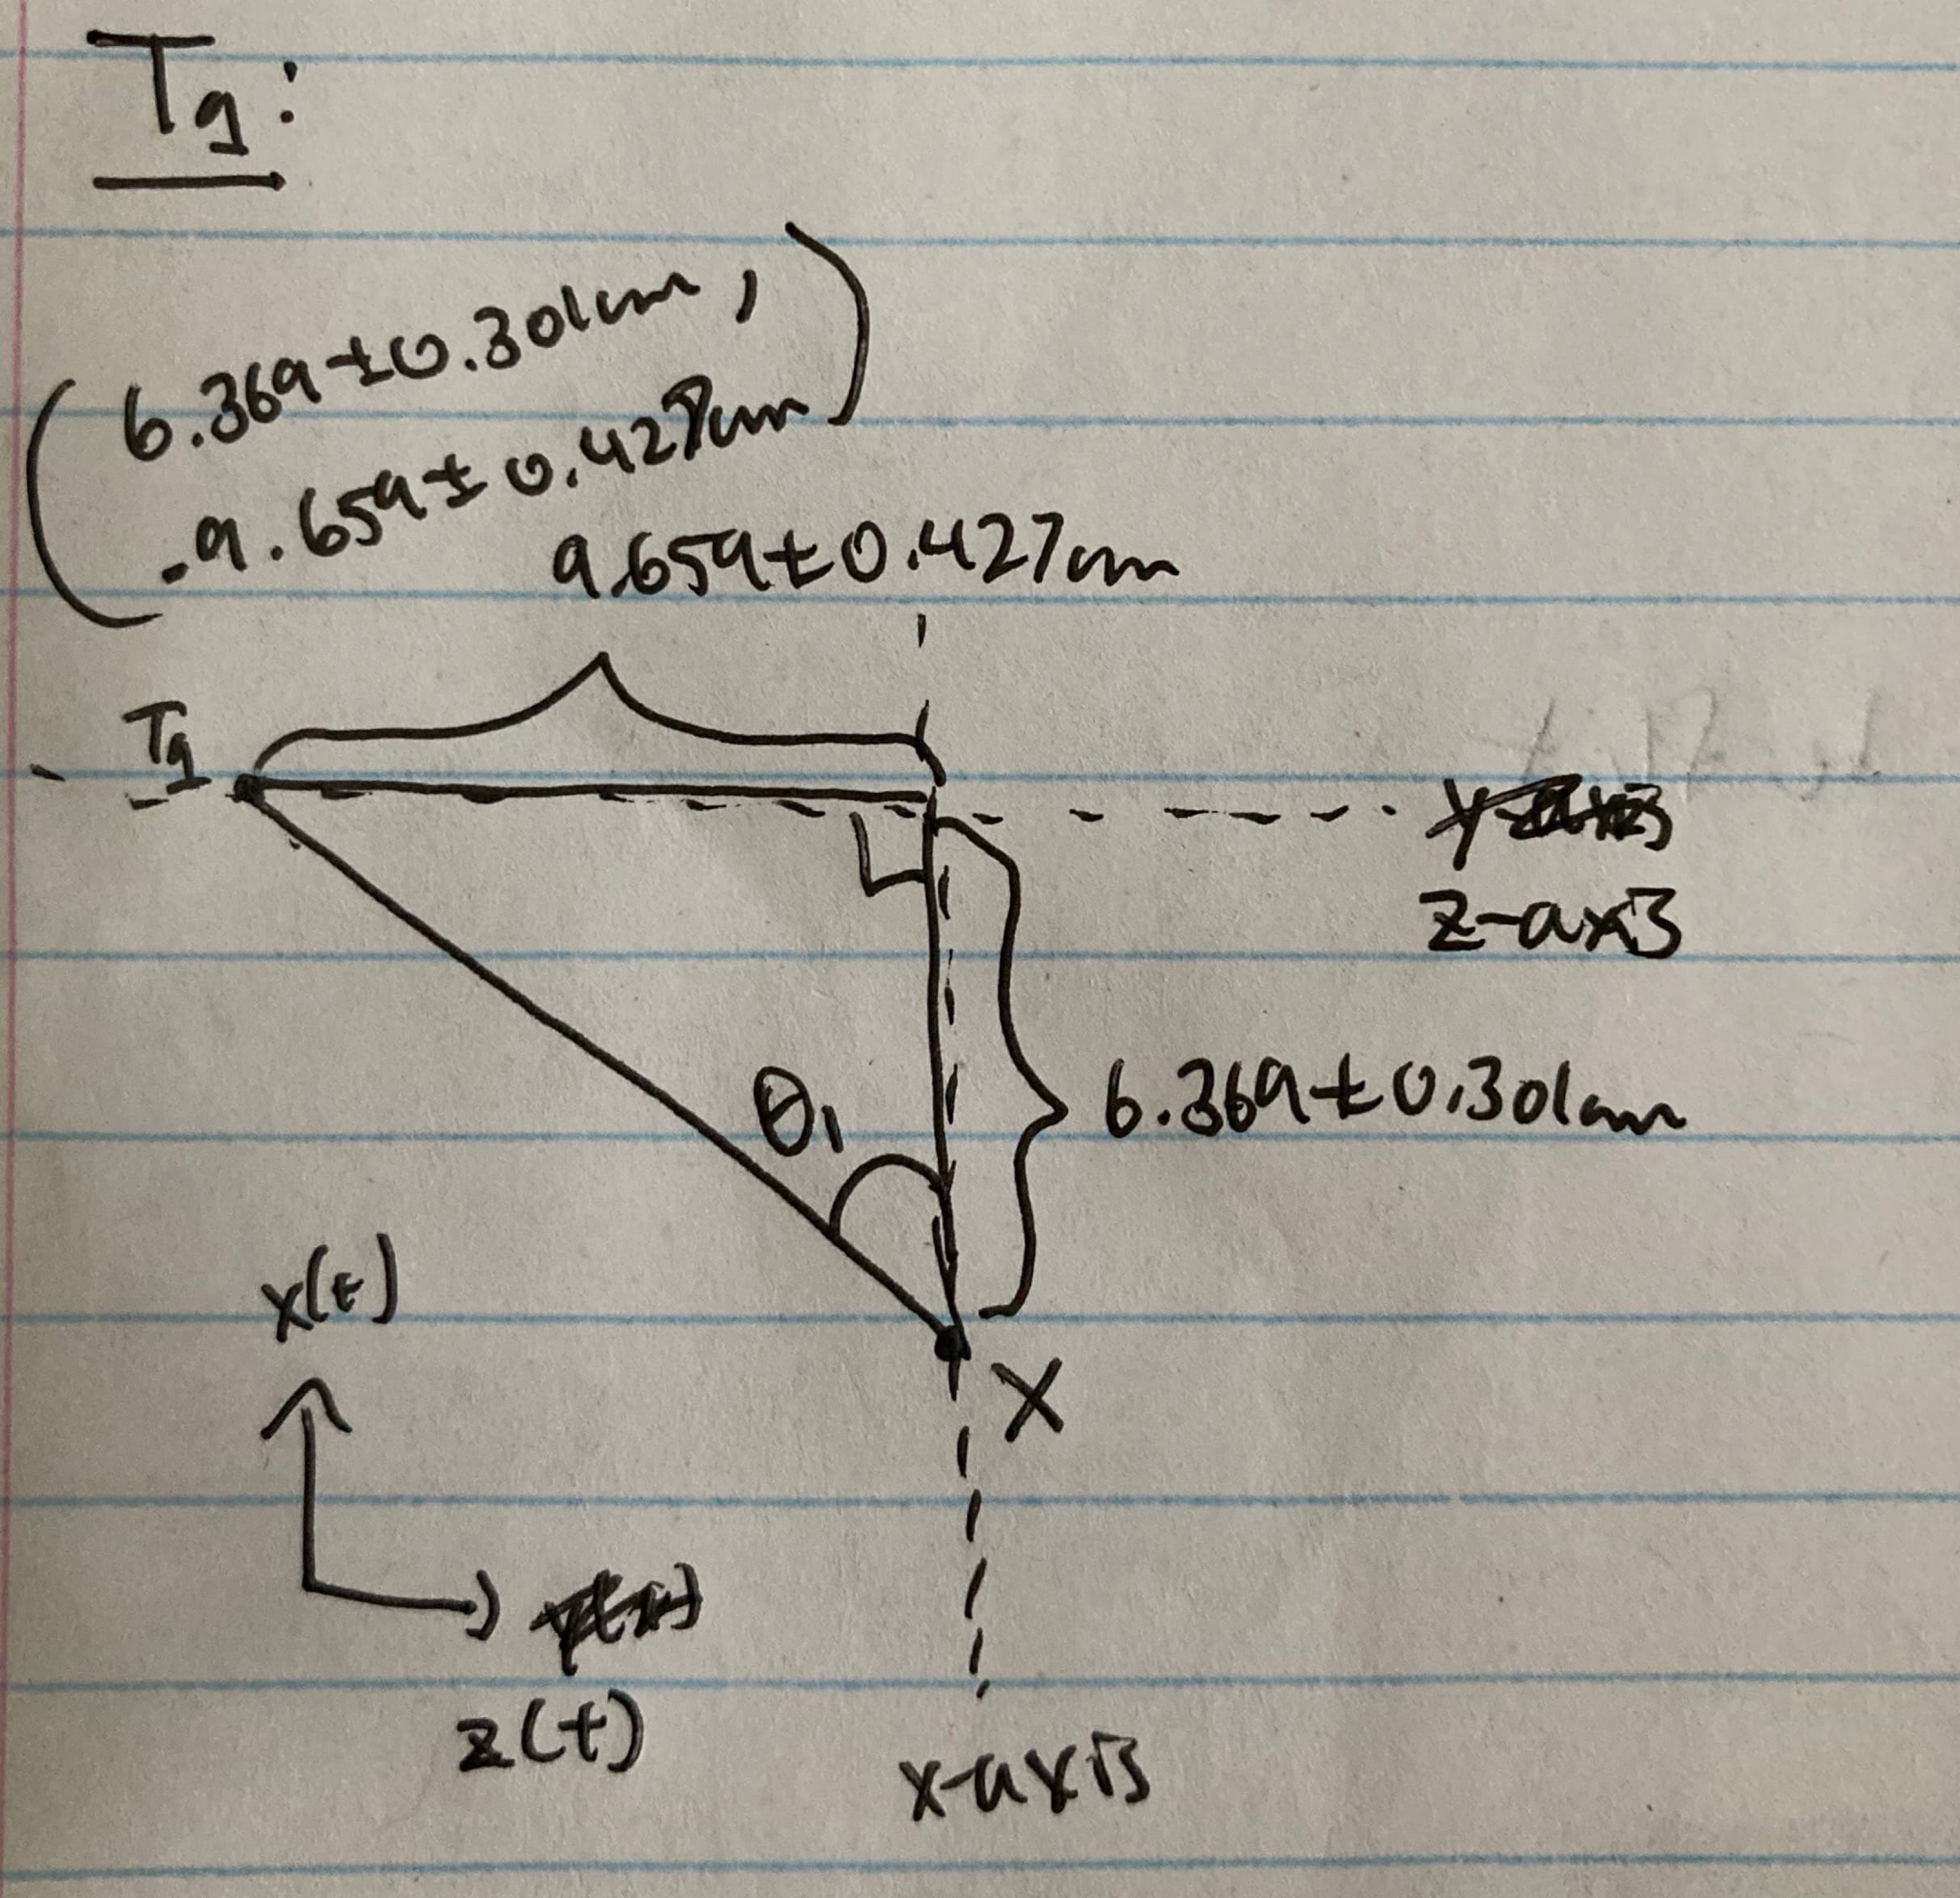
\includegraphics[width=0.4\textwidth]{T1Diagram.jpg}}} & 
{$\!\begin{aligned}
\theta{}_{T_{1}} &= \arctan{(\ce{\frac{T_{1y}}{T_{1x}}})}\\
&= \arctan{(\frac{9.659\pm0.427cm}{6.369\pm0.301cm})}\\
&= \arctan{(\frac{9.659cm\pm4.42\%}{6.369cm\pm4.73\%})}\\
&= \arctan{(1.516...\pm9.15\%)}\\
&\ce{Find uncertainty after arctan function}\\
&= 0.89785...\pm\frac{9.15\%/100\% \cdot{} 0.89785...}{1 + (0.89785...)^{2}}\\
&= 0.89785...\pm0.045485...rad\\
&= 0.90\pm0.04rad
\end{aligned}$}\\
\hline
\raisebox{-0.5\totalheight}{\fbox{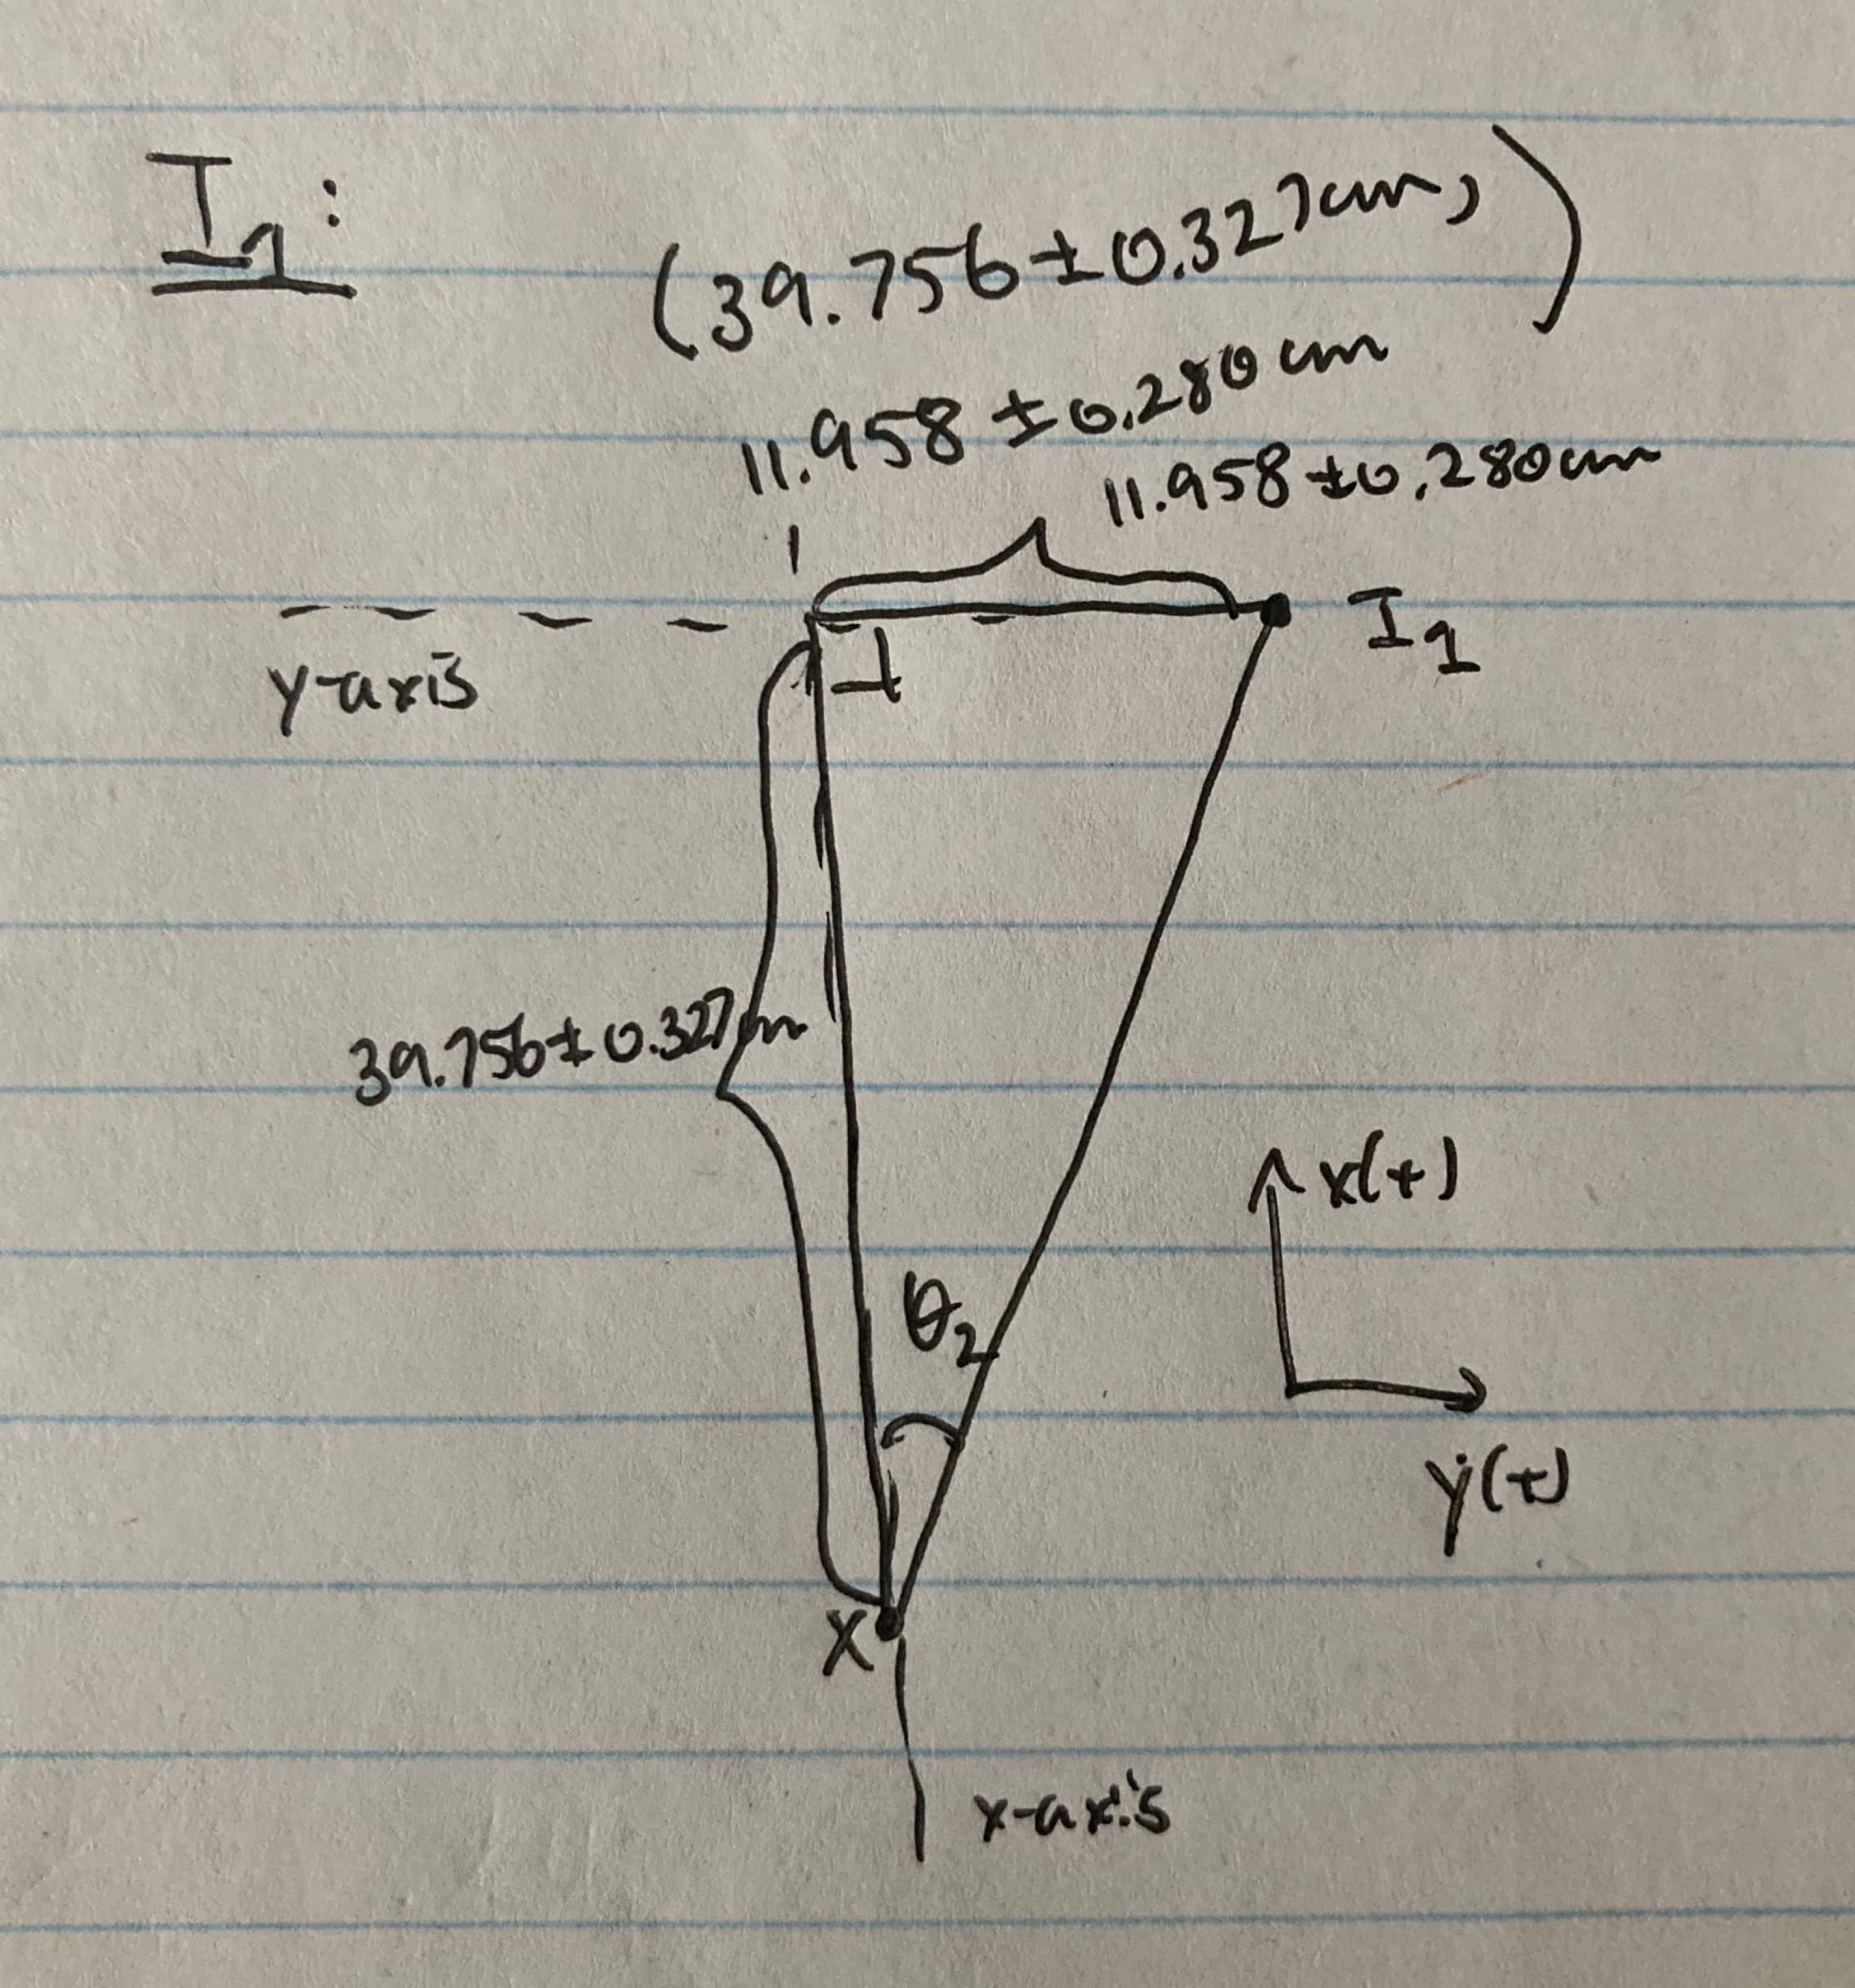
\includegraphics[width=0.4\textwidth]{I1Diagram.jpg}}} & 
{$\!\begin{aligned}
\theta{}_{I_{1}} &= \arctan{(\ce{\frac{I_{1y}}{I_{1x}}})}\\
&= \arctan{(\frac{11.958\pm0.280cm}{39.756\pm0.327cm})}\\
&= \arctan{(\frac{11.958cm\pm2.34\%}{39.756cm\pm0.823\%})}\\
&= \arctan{(0.3008...\pm3.163\%)}\\
&\ce{Find uncertainty after arctan function}\\
&= 0.2922...\pm\frac{3.163\%/100\% \cdot{} 0.2922...}{1 + (0.2922...)^{2}}\\
&= 0.2922...\pm0.00851...rad\\
&= 0.292\pm0.006rad
\end{aligned}$}\\
\hline
\end{tabular}
\end{center}


Therefore the angles between the line XT1 and x-axis is $0.90\pm0.04rad$ and line XI1 and x-axis is $0.292\pm0.006rad$.

\pagebreak

\subsection{Question 3}
Using your knowledge of the principle of conservation of energy and of projectile motion, determine the initial speed of the incident ball just before the collision as well as the final speed of both balls just after the collision. Show all proper equations and manipulations for full marks.

\subsubsection{Final Velocity of Incident Ball Right Before Collision (part 1)}
Find $v_{1}^{'}$ of $m_{1}$ at end of ramp where: $v_{1} = 0m/s$, $h_{1}^{'} = 0m$, $h_{1} = h_{table} = 75.5\pm0.1cm$, and where the system is defined as: $\ce{system} = \ce{m_{1} (ball 1) + ramp + earth + table}$

\begin{center}
\begin{tabular}{l|l}
\makecell{
$\!\begin{aligned}
\cancelto{0}{W_{ext}} + \cancelto{0}{W_{int,\ NC}} &= \triangle{}M_{sys}\\
M_{sys}^{'} &= M_{sys}\\
K_{1}^{'} + \cancelto{0}{U_{1}^{g'}} &= \cancelto{0}{K_{1}} + U_{1}^{g}\\
\frac{\cancel{m_{1}}(v_{1}^{'})^{2}}{2} &= \cancel{m_{1}}gh_{1}
\end{aligned}$\\\\
% new equations section
$\begin{aligned}
v_{1}^{'} &= \sqrt{2gh_{1}}\\
&= \sqrt{2 \cdot{} 9.8\cdot{}/s^2 \cdot{} (0.152m\pm0.658\%)}\\
&= \sqrt{2.979...m^2/s^2\pm0.658\%}\\
&= 1.726...m/s \pm 0.329\%\\
&= 1.726...m/s \pm 0.00561...m/s\\
&= 1.726...m/s \pm 0.006m/s\\
&= 1.726\pm0.006m/s
\end{aligned}$
% next left side calculations
} &
\makecell{
$\!\begin{aligned}
% solve for time with rel uncertainty
h_{1} &= 15.2\pm0.1cm\\
&= \frac{15.2cm}{100cm/m} \pm \frac{0.1cm\cdot{}100\%}{15.2cm}\\
&= 0.152m\pm0.658\%
\end{aligned}$\\\\\\\\
$\frac{1}{2} 0.658\% = 0.329\%$\\\\
$\frac{1.726...m/s \cdot{} 0.329\%}{100\%} = \pm0.00567m/s$
}
\end{tabular}
\end{center}

Therefore the velocity of $m_{1}$ at the end of the ramp is $v_{1}^{'} = 1.726\pm0.006m/s$

\pagebreak

\subsubsection{Solve for Free Fall Time}
Find the free fall time/duration for the balls.

\begin{center}
\begin{tabular}{c|c}
\raisebox{-0.5\totalheight}{\fbox{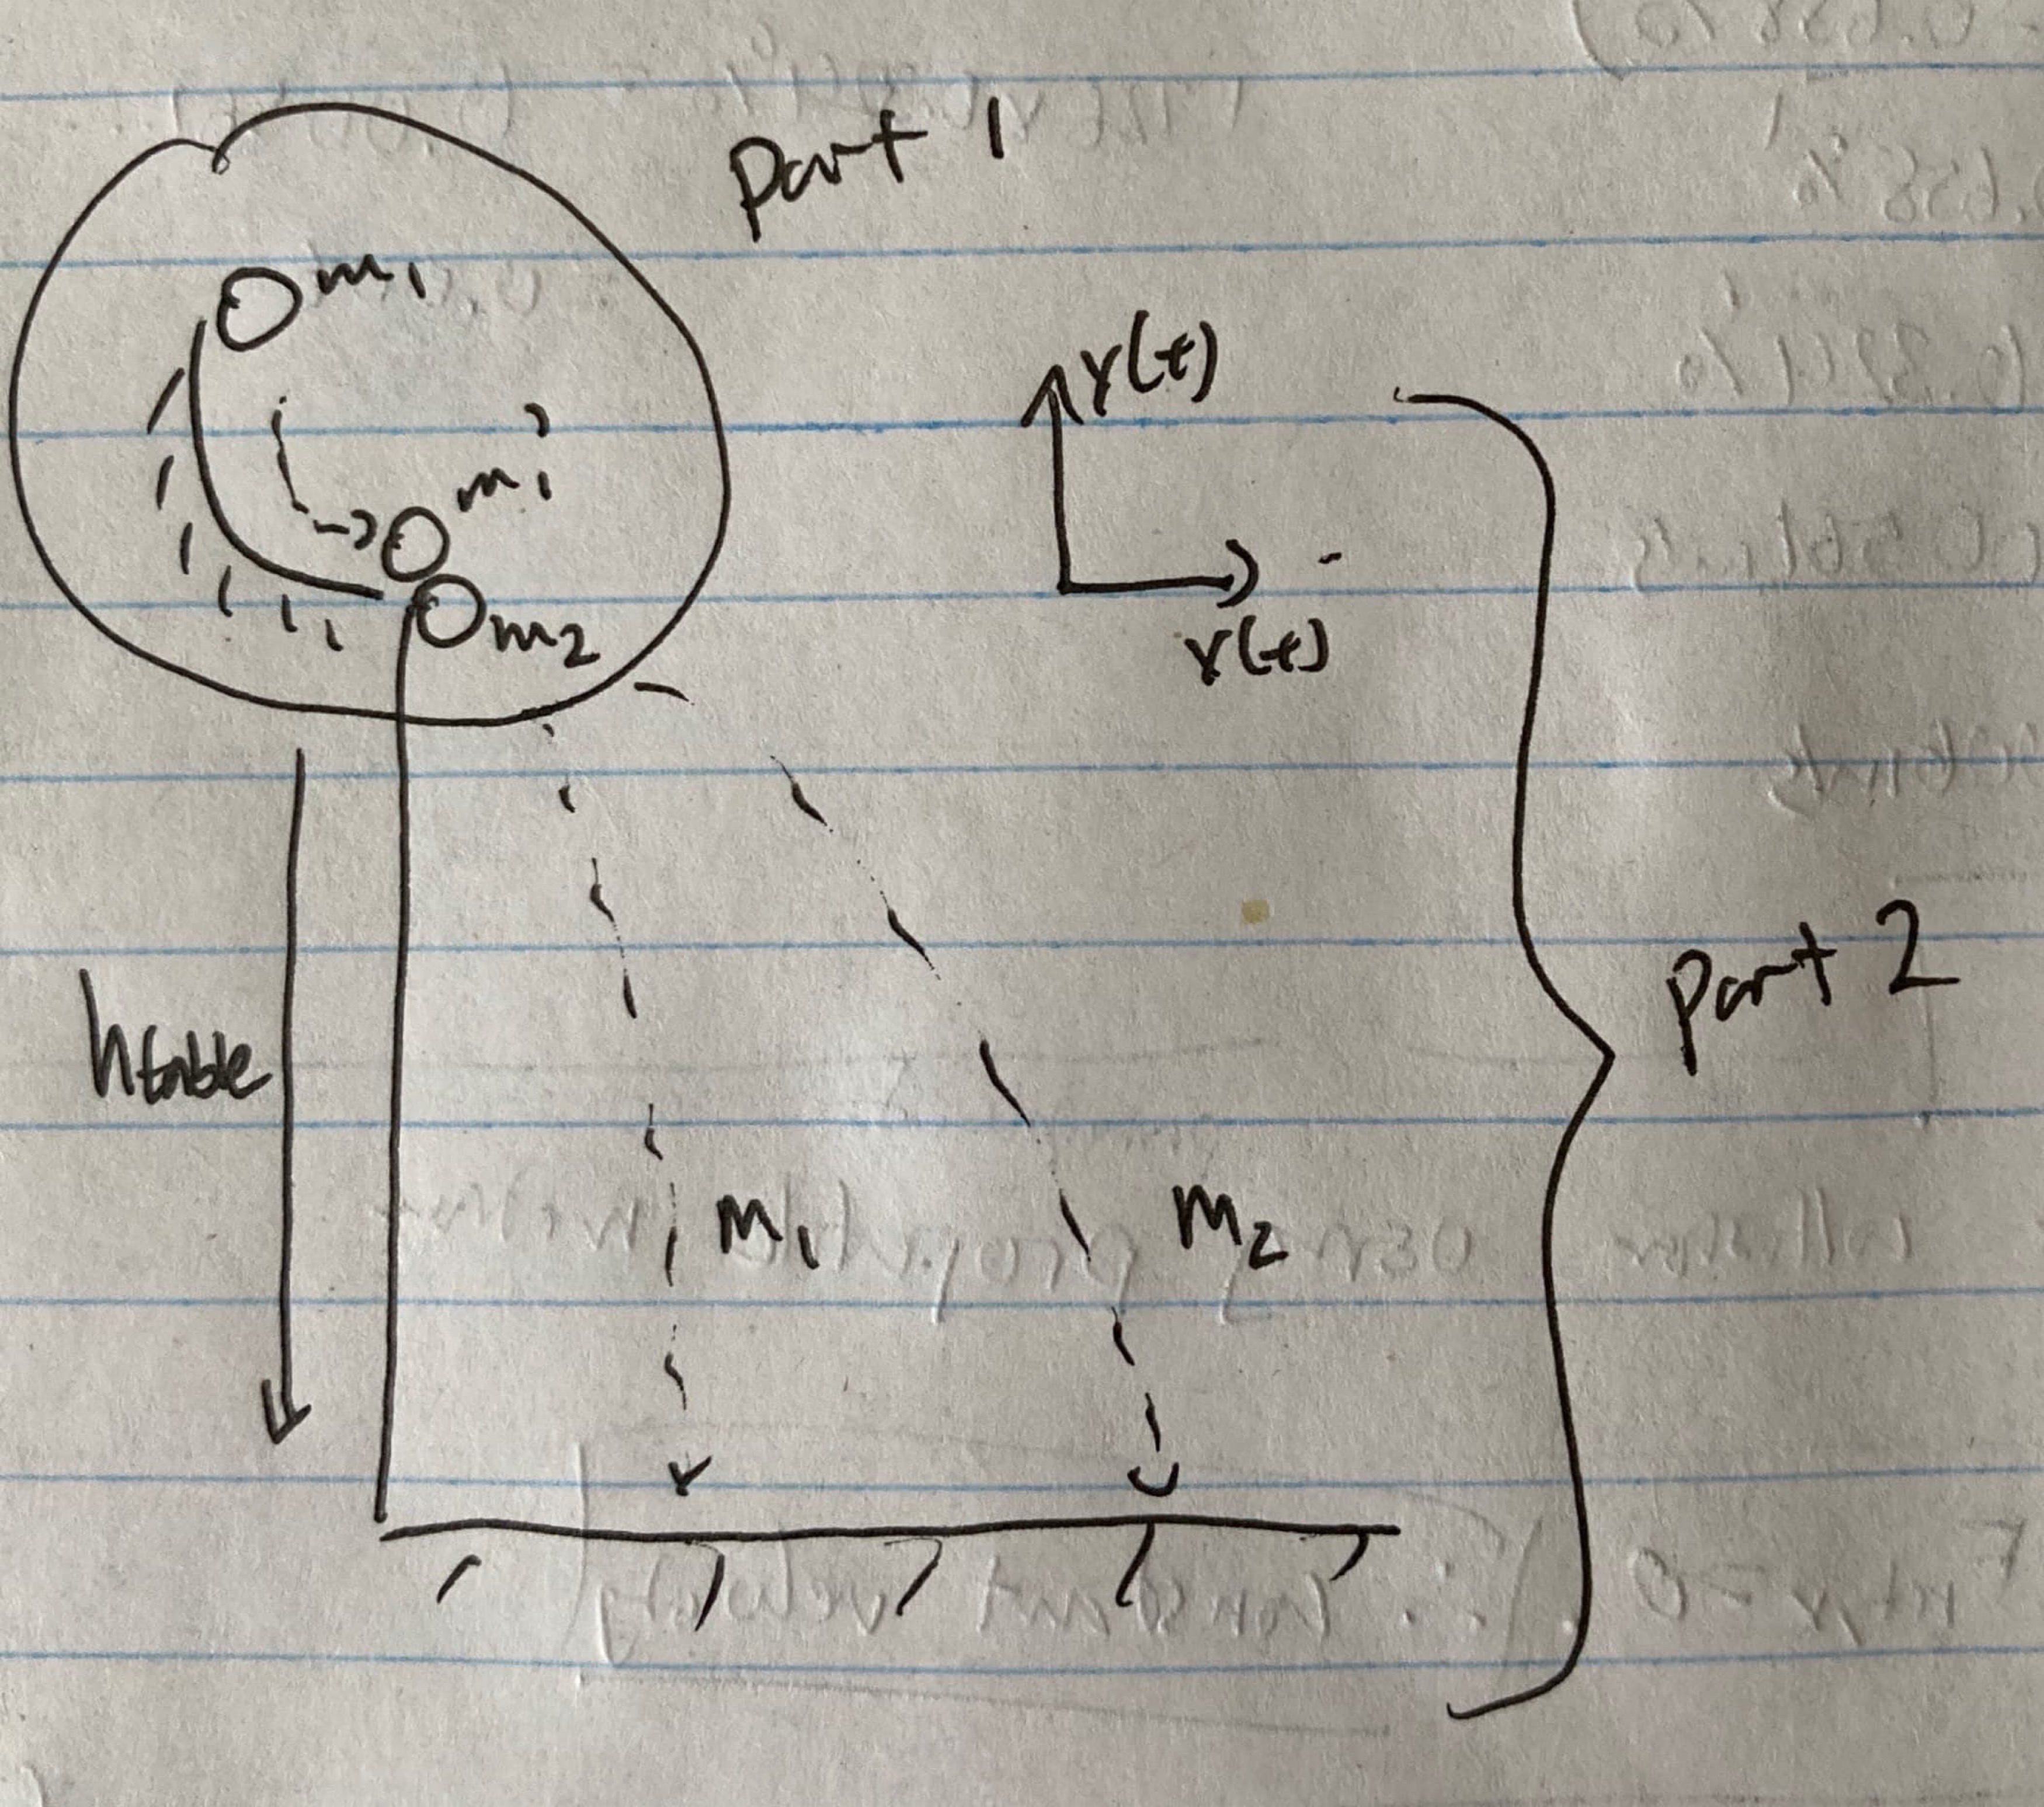
\includegraphics[width=0.4\textwidth]{HeightDiagram.jpg}}}
& \makecell{$\!\begin{aligned}
\triangle{y} &= \cancelto{0}{v_{y}\triangle{t}} + \frac{a_{y}(\triangle{t})^{2}}{2}\\
\triangle{t} &= \sqrt{\frac{2\triangle{y}}{a_{y}}}\\
\end{aligned}$}\\\\
% below image
\makecell{$\!\begin{aligned}
\triangle{t} &= \sqrt{\frac{2 \cdot{} (-75.5cm\pm0.1cm)}{-9.8m/s^{2}}}\\
&=\sqrt{\frac{2\cdot{}(-0.755m\pm0.132\%}{-9.8m/s^{2}}}\\
&= \sqrt{0.154s^{2} \pm 0.132\%}\\
&= \pm (0.3925...s\pm 0.066\%)\\
&= \pm (0.3925...s\pm 0.000259...s)\\
&= \pm (0.3925s\pm0.0003s)\\
& \ce{\triangle{t} cannot be negative}\\
\triangle{t} &= 0.3925\pm0.0003s
\end{aligned}$}
& \makecell{$\!\begin{aligned}
% convert cm to m
-75.5\pm0.1cm &= \frac{-75.5cm}{100cm/m} \frac{0.1cm\cdot{}100\%}{75.5cm}\\
&= -0.755m\pm0.132\%\\\\
\frac{1}{2} \cdot{} 0.132\% &= 0.066\%\\
\frac{0.066\% \cdot{} 0.3925...s}{100\%} &= 0.000259...s\\\\\\\\
\end{aligned}$}\\
\hline
\end{tabular}\end{center}

Thus, the time it takes for the balls to fall from a height of $h_{table} = 75.5\pm0.1cm$ is \fbox{$\triangle{t}_{table\rightarrow ground} = 0.3925\pm0.0003s$} by principle of projectile motion.

\pagebreak

\subsubsection{Final Velocity of Both Balls After Collision (part 2)}
Find $v_{1}^{'}$ and $v_{2}^{'}$ after collision using \textbf{principle of projectile motion}. Since the balls experience projectile motion after colliding, $\sum{F_{net,x}} = 0N$, and thus:\\\fbox{velocity in z-plane is constant in x direction (directly towards target point)}.


\begin{center}\begin{tabular}{l|l}
\ce{Find for Velocity of m_{1}}&\\
\makecell{
	$\!\begin{aligned}
\triangle{d}_{X\rightarrow T_{1}} = \triangle{d}_{1} &= v_{1}^{'}\triangle{t} + \cancelto{0}{\frac{a(\triangle{t})^{2}}{2}}\\
11.4\pm0.1cm &= v_{1}^{'}\triangle{t}\\
0.114m\pm0.877\% &= v_{1}^{'} (0.3925s\pm0.066\%)\\
	\end{aligned}$\\\\
% solve for v
	$\!\begin{aligned}
v_{1}^{'} &= \frac{0.114m\pm0.877\%}{0.3925s\pm0.066\%}\\
&= 0.36687m/s \pm 0.943\%\\
&= 0.36687m/s \pm 0.00345...m/s\\
&= 0.36687m/s \pm 0.003m/s\\
&= 0.367\pm0.003m/s\\
\vec{v_{1}^{'}} &= 0.367\pm0.003m/s [0.90\pm 0.04rad\\& \ce{above x-axis in z-plane]}
	\end{aligned}$\\
} &
\makecell{
$\!\begin{aligned}
% uc for distance
11.4\pm0.1cm &= \frac{11.4cm}{100cm/m} \pm \frac{0.1cm \cdot{} 100\%}{11.4cm}\\
&= 0.114m\pm0.877\%
\end{aligned}$\\\\\\\\
$\!\begin{aligned}
&= \frac{0.36687...m/s \cdot{}  0.943\%}{100\%}\\
&= \pm0.00345...m/s
\end{aligned}$
}\\
\hline
% section 
\ce{Find for Velocity of m_{2}}&\\
\makecell{
	$\!\begin{aligned}
\triangle{d}_{X\rightarrow I_{1}} = \triangle{d}_{2} &= v_{2}^{'}\triangle{t} + \cancelto{0}{\frac{a(\triangle{t})^{2}}{2}}\\
40.4\pm0.1cm &= v_{2}^{'}\triangle{t}\\
0.404m\pm0.247\% &= v_{2}^{'} (0.3925s\pm0.066\%)\\
	\end{aligned}$\\\\
% solve for v
	$\!\begin{aligned}
v_{2}^{'} &= \frac{0.404m\pm0.247\%}{0.3925s\pm0.066\%}\\
&= 1.0292...m/s \pm 0.313\%\\
&= 1.0292...m/s\pm 0.00322...m/s\\
&= 1.0292...m/s\pm 0.003m/s\\
v_{2}^{'} &= 1.029\pm 0.003m/s\\
\vec{v_{2}^{'}} &= 1.029\pm0.003m/s [0.292\pm0.006rad\\& \ce{below x-axis in z-plane]}
	\end{aligned}$\\
} &
\makecell{
$\!\begin{aligned}
% uc for distance
40.4\pm0.1cm &= \frac{40.4cm}{100cm/m} \pm \frac{0.1cm \cdot{} 100\%}{40.4cm}\\
&= 0.404m\pm0.247\%
\end{aligned}$\\\\\\\\
$\!\begin{aligned}
&= \frac{1.0292...m/s \cdot{}  0.313\%}{100\%}\\
&= \pm0.00322....m/s
\end{aligned}$
}\\
\hline
\end{tabular}\end{center}

\pagebreak

% final answer for q 3
The velocity of the incident ball just before collision is $v_{1}^{'} \ce{(part 1)} = 1.726\pm0.006m/s$ and the velocities of the two balls right after collision is $\vec{v_{1}^{'}} \ce{(part 2)} = 0.367\pm0.003m/s\ [0.90\pm0.04rad\ \ce{above x-axis in z-plane}]$ and $\vec{v_{2}^{'}} \ce{(part 2)} = 1.029\pm0.003m/s\ [0.292\pm0.006rad\ \ce{below x-axis in z-plane}$.



\subsection{Question 4}
Based on your calculations, is momentum conserved in the 2D collision? Justify. Show all equations and work for full marks.

\subsubsection{Conservation of Momentum}
Using Conservation of Momentum with the system defined as:\\
\textbf{system = $m_{1}$ (ball 1) + $m_{2}$ (ball 2)}

Since $F_{g} = F_{N}$ and no friction in both balls, $\sum{\vec{F_{ext}}} = 0$ and thus:\\

\begin{align*}
\cancelto{0}{\sum{\vec{F_{ext}}}} &= \frac{\vec{\triangle{P}_{sys}}}{\triangle{t}}\\
\vec{P_{sys}^{'}} &= \vec{P_{sys}}\\
\vec{p_{1}^{'}} + \vec{p_{2}^{'}} &= \vec{p_{1}} + \cancelto{0}{\vec{p_{2}}}\\
\vec{p_{1}^{'}} + \vec{p_{2}^{'}} &= \vec{p_{1}}
\end{align*}

Since conservation of momentum occurs in all direction (x-axis, y-axis, z-axis), solving for just the x-axis will suffice.

$$\therefore{} p_{1,x}^{'} + p_{2,x}^{'} = p_{1,x}$$

\pagebreak

\subsubsection{Component Form For Velocity Vectors}
Relative uncertainty for velocities is taken from previous calculations.

\begin{center}
\begin{tabular}{l|l}
\ce{Solving for $\vec{v_{1,x}^{'}}$}&\\

\makecell{$\!\begin{aligned}
% solving for x comp
v_{1,x}^{'} &= v_{1}\cdot{}\cos{\theta{}_{1}^{'}}\\
&= (0.367\pm0.003m/s)\cdot{}\cos{(0.90\pm0.04rad)}\\
&= (0.367m/s\pm0.943\%)[0.6216\pm(0.04 \cdot{} (0.6216...)]\\
&= (0.367m/s\pm0.943\%)[0.6216\pm0.0248...]\\
&= (0.367m/s\pm0.943\%)[0.6216\pm4\%]\\
&= 0.228...m/s\pm4.943\%\\
&= 0.228...m/s\pm0.0112...m/s\\
v_{1,x}^{'} &= 0.23\pm0.01m/s
\end{aligned}$} & \makecell{
\\\\
\\
$\frac{0.0248\cdot{}100\%}{0.6216} = 4\%$\\
$\frac{4.943\%\cdot{}0.228m/s}{100\%} = 0.0112...m/s$\\
}\\
\\
\ce{Solving for $\vec{v_{2,x}^{'}}$}&\\

\makecell{$\!\begin{aligned}
% solving for x comp
v_{2,x}^{'} &= v_{2}\cdot{}\cos{\theta{}_{2}^{'}}\\
&= (1.029\pm0.003m/s)\cdot{}\cos{(-0.292\pm0.06rad)}\\
&= (1.029m/s\pm0.313\%)[0.9576\pm(0.06 \cdot{} (0.9576...)]\\
&= (1.029/s\pm0.313\%)[0.9576\pm0.05746...]\\
&= (1.029/s\pm0.313\%)[0.9576\pm6\%]\\
&= 0.9853...m/s\pm6.313\%\\
&= 0.9853...m/s\pm0.0622...m/s\\
v_{2,x}^{'} &= 0.99\pm0.06m/s
\end{aligned}$} & \makecell{
\\\\
\\
$\frac{0.0574...\cdot{}100\%}{0.9576} = 6\%$\\
$\frac{6.313\%\cdot{}0.9853m/s}{100\%} = 0.0622...m/s$\\
}\\
\\
\\
$v_{1,x}$ is already known to be $v_{1,x} = 1.726\pm0.006m/s$
\end{tabular}
\end{center}

\pagebreak
\subsubsection{Check if Momentum is Conserved}
Since the balls have same mass, $m_{1} = m_{2} = m$

\begin{center}
\begin{align*}
p_{1,x}^{'} + p_{2,x}^{'} &= p_{1,x}\\
m_{1}\cdot{}v_{1,x}^{'} + m_{2}\cdot{}v_{2,x}^{'} &= m_{1}\cdot{}v_{1,x}\\
\cancel{m}\cdot{}v_{1,x}^{'} + \cancel{m}\cdot{}v_{2,x}^{'} &= \cancel{m}\cdot{}v_{1,x}\\
v_{1,x}^{'} + v_{2,x}^{'} &= v_{1,x}\\
(0.228\pm0.0112m/s) + (0.985\pm0.0622m/s) &= (1.726\pm0.006m/s)\\
(1.213\pm0.0734m/s) &= (1.726\pm0.006m/s)\\
\end{align*}
\end{center}

$\therefore{}$ the left side is not equal to the right side and the uncertainties do not overlap, thus \fbox{the momentum is not conserved in 2D.}


\pagebreak
\subsection{Question 5}
Based upon your calculations, is the collision, (perfectly) elastic or not? Justify. Show all equations and work for full marks.

Using Conservation of Energy and the system is defined as: \textbf{system = $m_{1}$ + $m_{2}$ + ramp + earth + table}. Thus the equation is defined as:

\begin{center}\begin{align*}
\cancelto{0}{W_{ext}} + \cancelto{0}{W_{int, NC}} &= \triangle{M}_{sys}\\
M_{sys}^{'} &= M_{sys}\\
\end{align*}\end{center}

An elastic collision is when \fbox{$\triangle{Q} = \triangle{U} + \triangle{E}_{th} = 0$}. Thus, assuming $\triangle{Q} = 0$, $Q^{'} = Q$. Furthermore, the initial state of the system will be (part 1) and the final state is (part 2) and values will be taken from previous calculations.

\begin{center}\begin{align*}
K_{1}^{'} + K_{2}^{'} + Q^{'} &= K_{1} + K_{2} + Q\\
\ce{Since Q^{'} &= Q}\\
K_{1}^{'} + K_{2}^{'} &= K_{1} + \cancelto{0}{K_{2}}\\
\frac{m_{1}(v_{1}^{'})^{2}}{\cancel{2}} + \frac{m_{2}(v_{2}^{'})^{2}}{\cancel{2}} &= \frac{m_{1}(v_{1})^{2}}{\cancel{2}}\\
\ce{Since balls have same mass, m_{1} = m_{2} = m}&\\
\cancel{m}\cdot{}(v_{1}^{'})^{2} + \cancel{m}\cdot{}(v_{2}^{'})^{2} &= \cancel{m}\cdot{}(v_{1})^{2}\\
(v_{1}^{'})^{2} + (v_{2}^{'})^{2} &= (v_{1})^{2}\\
(0.367\pm0.003m/s)^{2} + (1.029\pm0.003m/s)^{2} &= (1.726\pm0.006m/s)^{2}\\
[0.13469...\pm(2\cdot{}0.003)m^{2}/s^{2}] + [1.05884...\pm(2\cdot{}0.003)m^{2}/s^{2}] &= [2.979...\pm(2\cdot{}0.006)m^{2}/s^{2}]\\
(0.13469...\pm0.006m^{2}/s^{2}) + (1.05884...\pm0.006m^{2}/s^{2}) &= (2.979...\pm0.012m^{2}/s^{2})\\
(1.19353...\pm0.012m^{2}/s^{2}) &= (2.979...\pm0.012m^{2}/s{2})\\
\ce{LS \neq RS}& \therefore{} U \neq 0\\
\end{align*}\end{center}
\pagebreak
Since the kinetic energy is not conserved, $\triangle{U}\neq0$. From the data shown above, the uncertainties do not overlap and LS < RS. Since the final mechanical energy is less than the initial, $\triangle{U} = U^{'} - U$ where $U^{'} > U$. \\\fbox{$\therefore{\triangle{U} > 0}$ and the collision \textbf{inelastic} and the collision is not elastic!}


\subsection{Question 6}
Give at least 2 sources of error in this lab.

\subsubsection{Friction}
Air friction and rolling friction were not accounted for which will affect the final result.

\subsubsection{Imperfect Setup}
In the experiment, the Ramp may not have been perfectly aligned with the X-axis which will affect calculated angles and momentum values.







\end{document}
